\documentclass{article}
% if you need to pass options to natbib, use, e.g.:
    \PassOptionsToPackage{numbers}{natbib}
% before loading neurips_2023

\usepackage[preprint]{neurips_2023}

\usepackage[utf8]{inputenc} % allow utf-8 input
\usepackage[T1]{fontenc}    % use 8-bit T1 fonts
\usepackage{hyperref}       % hyperlinks
\usepackage{url}            % simple URL typesetting
\usepackage{booktabs}       % professional-quality tables
\usepackage{amsfonts}       % blackboard math symbols
\usepackage{nicefrac}       % compact symbols for 1/2, etc.
\usepackage{microtype}      % microtypography
\usepackage{xcolor}         % colors
\usepackage{graphicx}
\usepackage{float}
\usepackage{listings}

\title{Current Topics in Digital Philology --- \\Assignment 6: Digital Methods in Literary Analysis}

\author{%
  Daan Brugmans \\
  Radboud University\\
  \texttt{\url{daan.brugmans@ru.nl}} \\
}

\begin{document}

\bibliographystyle{plainnat}

\maketitle

\section{Introduction}
In this small-scale study, I explore the use of digital methods for a stylometric comparison between the written works of multiple authors.
Specifically, I analyze how different aspects of authors' writing styles featured in NLTK's subset of the Gutenberg Corpus influence the decision making of a machine learning model.
This model is trained to classify an input text to an author using a set of features that are based on the writing style used in the text to be classified.
This way, the model learns to classify a text to its author using the style of the text's author.
The task of classifying a text to an author is called authorship attribution.
Once the model is trained, an ablation study is performed to gain an insight into which features the model finds the most useful.
Since these features are based on stylistic characteristics of the texts, such an ablation study shows which aspects of an author's writing style contain the most extractable information when trying to attribute a text to an author, or in other words, which parts of an author's writing style are most useful to look at.

\section{Related Work}
There already exists a significant body of work on the topic of authorship attribution and the use of digital methods for this task.
Stamatatos \cite{stamatatos2009surveymodern,stamatatos2016authorshipverification} provides an overview of such methods and stylometric features.
Specifically, Stamatatos shows how different types of stylometric features can be used for the authorship attribution task, such as lexical features that describe a text's quantitative metadata, syntactic features that give insight in how an author constructs sentences and the (often subconscious) choices involved in that process, and semantic features that tell something about the contents of the texts an author writes.
They also describe two main approaches to an authorship attribution setup: profile-based approaches, where all texts of an author are grouped into one profile and the profiles are compared against a text with an unknown author, and instance-based approaches, where smaller, individual texts are labelled as belonging to an author and a classification model is trained on these texts so that it can be used to attribute an author to a text whose author is unknown.
My study is an example of an instance-based approach using a machine learning model as a classifier.

For the purpose of this research, there are a few metrics proposed in different works that are used as features for the machine learning model.
The \textit{Lexical Diversity Coefficient} is a metric proposed by Hlavcheva et al. \cite{hlavcheva2021languageindependentfeatures} that aims to describe the lexical diversity of a text by computing the amount of unique words over the total amount of words.
This gives a relative value that describes the share of words that occur only once in a text.
Hess et al. \cite{hess1989reliabilitytypetoken} describe a similar metric called \textit{Herdan's Log Type Token Richness}, which is computed by taking the log of the amount of unique words in a text over the log of the total amount of words in a text.

Additionally, Hlavcheva et al. also describe their \textit{Syntactic Complexity Coefficient} metric.
This metric is computed by taking the total amount of sentences in a text over the total amount of words in a text, and subtracting that value from 1.
This gives a metric that ranges from 0 to 1, where a higher number means that the overall syntactic complexity of the text is higher; for example, if the total amount of words used in a text remains the same, but the number of sentences used goes down, then the sentences in the text have become longer, which makes the text more syntactically complex.

\section{Methods}
I used NLTK's subset of the Gutenberg corpus as a dataset.
It contains eighteen different historical literary works from a variety of authors.
Out of the authors included in this dataset, three have at least two different works included:
\begin{itemize}
  \item \textbf{William Shakespeare}: \textit{The Tragedy of Julius Caesar}, \textit{Hamlet}, and \textit{Macbeth}.
  \item \textbf{Jane Austen}: \textit{Emma}, \textit{Persuasion}, and \textit{Sense and Sensibility}.
  \item \textbf{Gilbert Keith Chesterton}: \textit{The Ball and the Cross}, a collection of stories about \textit{Father Brown}, and \textit{The Man Who Was Thursday}.
\end{itemize}
I have used these nine works as part of my research, foregoing the use of the other works.
I made this decision on the basis that this way, I can split different works from the same author across multiple data splits for the machine learning setup.
Although I could use the other works included in the Gutenberg corpus too, I would have to split these individual works across multiple data splits, and I did not want to do that because that could enable the machine learning model to learn to attribute an author to a text based on the information embedded in the work itself, instead of the style of the work.
By using whole works by the same author in different data splits, the model cannot use the information embedded in an individual work's contents to attribute an author, so it will have to look across multiple works by the same author.
% This decision was motivated by how this distribution of data would align with the problem at hand: with a dataset of three separate textual works for every author, for three different authors total, a dataset can be constructed where splits for a train, validation, and test set all contain one literary work per author.
This would be especially relevant for models that learn their own features, such as neural networks.
However, for the sake of this study and its setup, I have used a traditional machine learning model without doing any hyperparameter optimization, and I do not use a validation split for that reason.
The works used are split accordingly:
\begin{itemize}
  \item \textbf{Train}: \textit{The Tragedy of Julius Caesar} and \textit{Hamlet} by William Shakespeare, \textit{Emma} and \textit{Persuasion} Jane Austen, and \textit{The Ball and the Cross} and \textit{Father Brown} by G. K. Chesterton.
  \item \textbf{Test}: \textit{Macbeth} by Shakespeare, \textit{Sense and Sensibility} by Austen, and \textit{The Man Who Was Thursday} by Chesterton.
\end{itemize}

Out-of-the-box, this data provided by the Gutenberg corpus can't be used for a machine learning environment, since that would make every work an individual data point.
That is why I split the contents of the works into smaller data points that can be used for training and evaluation.
Specifically, the Gutenberg corpus offers the works on a per-sentence basis.
For every work, I create groups of 5 sentences, forming a (small) paragraph, and consider that a single data point.
The choice of 5 sentences per data point is a hyperparameter, and a further exploration of this study could search for a more optimal value.
Increasing the amount of sentences in a data point would produce data points containing more information, but would decrease the amount of data points to train on, while decreasing this number does the opposite.
I chose to go with 5 since I thought this would strike a good balance between having enough data points to train on, and having data points that contained enough textual information to extract meaningful and useful features.
The size of the resulting dataset and the distribution of its data across authors and splits is shown in table \ref{tab:dataset}.

\begin{table}[]
\centering
\begin{tabular}{l|lll|l}
                & \textbf{Shakespeare} & \textbf{Austen} & \textbf{Chesterton} & \textbf{Total} \\ \hline
  \textbf{Train} & 1055                 & 2301            & 1718                & 5074           \\
  \textbf{Test}  & 382                  & 1000            & 749                 & 2131           \\ \hline
  \textbf{Total} & 1437                 & 3301            & 2467                & 7205          
\end{tabular}%
\caption{The amount and distribution of data points in the final dataset used to train the machine learning model, on the basis of 5 sentences of a work's text as a single data point. Rows show splits, columns show authors.}
\label{tab:dataset}
\end{table}

I chose to train an XGBoost model \cite{chen2016xgboost}, trained using the default hyperparameters provided by the XGBoost Python implementation, which is commonly used due to its good performance on many tasks that use manually created descriptive features.
I provided this model with a set of such descriptive features, which all aim to describe characteristics of the texts themselves or of the writing style used by the text's author.
For example, features such as Word Count and Sentence Count provide straightforward information about the text's quantitative metadata, features such as Mean Sentence Length, Hapax Legomenon Count, and Mean Word Frequency describe the text's complexity, features such as Contraction Count and Swear Count tell something about the author's choice of words and phrasing, and features such as He/She Ratio and the Sentiment Scores provide an insight into what kinds of works the author produces.
Alternatively, it could also be said that this list of descriptive features include lexical, syntactic, and semantic features, and the choice of these types of features align with the stylometric feature types described by Stamatatos et al. \cite{stamatatos2009surveymodern,stamatatos2016authorshipverification}. 
This specific set of features is directly based on a set of features I have used before in an authorship attribution setup and which proved to be useful.
The following is the list of features used by the model:
\begin{itemize}
  \item \textbf{All Caps Word Count}: the amount of words that are written using only capitalized letters.
  \item \textbf{Sentence without Capital at Start}: the amount of sentences in a data point that do not start with a capital letter.
  \item \textbf{Sentence Lower at Start}: the amount of sentences in a data point that start with a non-capitalized letter. This feature is separate from the prior one, as combination excludes counting sentences that start with something that isn't a letter.
  \item \textbf{A/An Error Count}: the amount of times that the use of ``a'' and ``an'' was not used properly in a data point.
  \item \textbf{Continuous Punctuation Count}: the amount of times a sentence in a data point ends with trailing periods (\dots).
  \item \textbf{Quotation Count}: the amount of times something is quoted using quotation marks.
  \item \textbf{Question Count}: the amount of times a sentence ends in a question mark.
  \item \textbf{Exclamation Count}: the amount of times a sentence ends in an exclamation mark.
  \item \textbf{He/She Ratio}: the ratio of the amount of times ``he'' is used in a data point over the amount of times ``she'' is used in a data point.
  \item \textbf{Character Count}: the amount of characters in a data point.
  \item \textbf{Word Count}: the amount of words in a data point.
  \item \textbf{Sentence Count}: the amount of sentences in a data point.
  \item \textbf{Punctuation Count}: the amount of punctuation occurrences in a data point.
  \item \textbf{Digit Count}: the amount of times a digit is written in a data point. Numbers consisting of multiple digits have all their digits counted.
  \item \textbf{Uppercase Count}: the amount of times uppercase characters are used in a data point.
  \item \textbf{Short Word Count}: the amount of times a ``short'' word was used in a data point. Here, a short word is defined as a word that consists of 4 characters or less.
  \item \textbf{Alphabet Count}: the amount of unique characters that are used in a data point.
  \item \textbf{Contraction Count}: the amount of times contractions such as ``don't'' are used in a data point.
  \item \textbf{Word Without Vowels Count}: the amount of times words without vowels are used in a data point. Here, the letter ``y'' is not considered a vowel.
  \item \textbf{Hapax Legomenon Count}: the amount of times a word is used in the data point that isn't used anywhere else in the data point.
  \item \textbf{Mean Word Length}: the mean length of words in a data point.
  \item \textbf{Mean Sentence Length}: the mean length of sentences in a data point.
  \item \textbf{Word Length Standard Deviation}: the standard deviation of the amount of words used in a data point.
  \item \textbf{Sentence Length Standard Deviation}: the standard deviation of the amount of sentences used in a data point.
  \item \textbf{Mean Word Frequency}: the mean amount of times a word is used in a text.
  \item The \textbf{Lexical Diversity Coefficient} \cite{hlavcheva2021languageindependentfeatures}.
  \item The \textbf{Syntactic Complexity Coefficient} \cite{hlavcheva2021languageindependentfeatures}.
  \item The \textbf{Herdan's Log Type Token Richness} \cite{hess1989reliabilitytypetoken}.
  \item \textbf{Sentiment Scores}: a sentiment analysis model assesses the sentiment of the data point to be either positive, negative, or neutral, and provides a relative score to all three options such that they all add to 1. These scores are then stored as their own feature: the \textbf{Positive Sentiment Score}, \textbf{Neutral Sentiment Score}, and \textbf{Negative Sentiment Score}. The sentiment analysis model used is ``twitter-roberta-base-sentiment'' by CardiffNLP \cite{barbieri2020tweeteval}.
  \item \textbf{Swear Word Count}: the amount of times swear words are used in a data point. Swear words are detected using the Python package ``better\_profanity'' \cite{nguyen2026snguyenthanhbetterprofanity}.
\end{itemize}

\section{Results}
After the model is trained, an ablation study is performed.
The study retrains the model on the same data, while using all of the features mentioned in the above list except one.
The resulting model is evaluated on the test dataset and it's F1-score is recorded, a balance between the model's precision and recall.
This is done for every feature of the dataset, until there are F1-scores for every feature being ablated.
These scores are compared to each other, with a focus on how much the F1-score dropped when a specific feature is ablated compared to other ablated features.
The more the F1-score drops when a specific feature is ablated, the more important information it contains that was used by the model to come to a correct prediction.
This means that ablated features with relatively low F1-scores contain more valuable information than those with higher F1-scores.
Figure \ref{fig:ablation} shows the results of the ablation study on the dataset as described in the Methods section.

Furthermore, the model trained on all features was also evaluated on the test set.
The overall classification accuracy of the model was recorded at 84.7\%, as well as the overall F1-score of 84.8\%.
The precision, recall, and F1-score per author was also recorded.
Figure \ref{tab:results} shows these per-author results.

\begin{table}
  \centering
  \begin{tabular}{l|lll}
                      & \textbf{Precision} & \textbf{Recall} & \textbf{F1-score} \\ \hline
  \textbf{Shakespeare}      & 98\%               & 99\%            & 99\%              \\
  \textbf{Austen}  & 87\%               & 80\%            & 83\%              \\
  \textbf{Chesterton} & 76\%               & 83\%            & 80\%             
  \end{tabular}
  \caption{Per-author precision, recall, and F1-scores for the model trained on all features.}
  \label{tab:results}
\end{table}

\begin{figure}
    \centering
    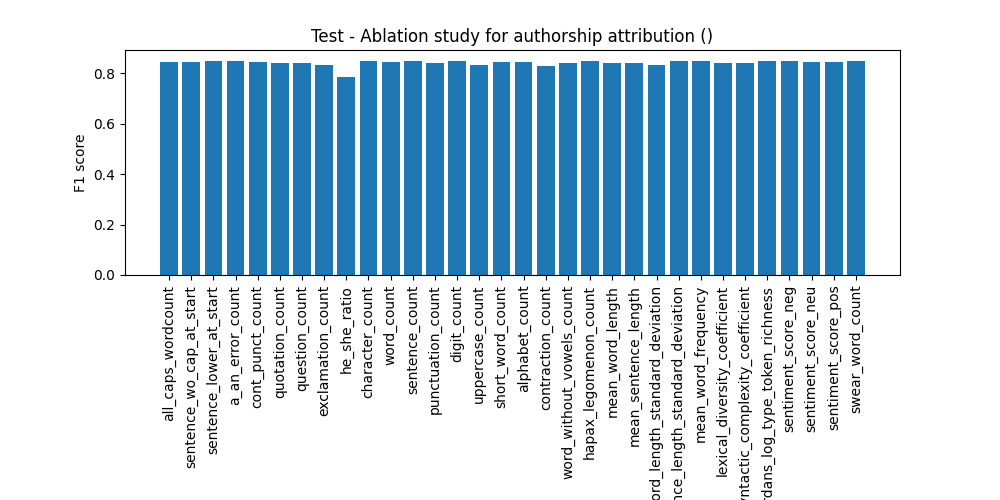
\includegraphics[width=\textwidth]{images/ablation_plot_test.png}
    \caption{Results of the ablation study.}
    \label{fig:ablation}
\end{figure}

\section{Discussion}
The results show an overall decent performance of the model on the trinary classification task.
The average accuracy achieved by the model is 84.7\%, which is well above randomly guessing, and the model seems to be able to recognize which author has written which text based on only stylistic features of the text.
The model performs best at classifying works from Shakespeare, achieving an F1-score of 99\%, with works by Austen and Chesterton achieving lower F1-scores.

The ablation study shows that most features are about as important to the model, as there is little difference between most of the ablated features.
One feature does show a noticeable drop in performance when removed from the set of features: the he/she ratio.
This means that out of the features used, the model gets the most information about the author's style in a single feature when that feature describes how the ratio of the usage of ``he'' and ``him'' over ``she'' and ``her'' is compared to the data it was trained on.
Although there are no other features that cause a dip in performance when ablated as much as the he/she ratio, there are some features that do slightly reduce performance.
These include the uppercase count, contraction count, and the word length standard deviation.
Excluding these features seems to have a larger effect on model performance than excluding the remaining features.

Within the field of digital humanities, this work serves as a small-scale example of how modern digital methods can be used to solve problems to levels of efficiency and efficacy that could not be achieved without modern digital methods.
The dataset used here contained only texts for which the author was already known.
However, the approach used in this report can be extended to texts whose author is unknown: by collecting a dataset of texts written by potential candidates of a text whose author is unknown, the form of authorship attribution used in this report can give quantitative predictions on the likelihood of any of the candidate authors being the unknown author.

\section{Conclusion}
In this report, I showed how machine learning methods can be used to analyze the writing style of different authors, specifically in how differences in writing styles can be learned by machine learning models to perform authorship attribution to texts with unknown authors.
I trained an XGBoost model on a dataset of literary works from William Shakespeare, Jane Adams, and Gilbert Keith Chesterton as an example of digital methods for authorship attribution.
This model achieved an overall accuracy of 84.7\%.
I also performed an ablation study to discover which of the stylistic features used by the model to make its predictions contains the most valuable information.
The results from this study show that the ratio of use of ``he'' and ``him'' over ``she'' and ``her'' are relied upon the most by the trained model.

\bibliography{refs}

\end{document}
